%!TEX program = xelatex

%-----------------------------导言区---------------------------%
	\documentclass[10pt,oneside,UTF8]{book}
	\usepackage[fontset=mac]{ctex}
	\usepackage[shortlabels]{enumitem}
	\usepackage{graphicx,subfigure,booktabs,multirow,caption,setspace,listings,amsmath,amsfonts,lineno,multicol,float,stfloats}  % 直接导入常用包
	\usepackage{xcolor,colortbl,rotating,bigstrut}
	\usepackage{hyperref} % 生成书签和超链接
	\usepackage{ulem} %解决文字下划线无法自动换行的问题(暂时无用)
	\usepackage[hyperref=true,backend=biber,bibstyle=gb7714-2015,citestyle=numeric-comp,sorting=none,backref=true]{biblatex}
	\usepackage{titlesec}
		%改变section、subsection里面字体的样式。中文黑体,英文TNR。
		\newfontfamily\sectionef{Times New Roman}
		\newcommand{\sectioncf}{\CJKfamily{FZHeiTi}}
		\titleformat*{\section}{\Large\bfseries\sectioncf\sectionef}
		\titleformat*{\subsection}{\large\bfseries\sectioncf\sectionef}
	\usepackage{fancyhdr}
	\usepackage{geometry} % 用于纸张格式的设置
	\geometry{a4paper,scale=0.85,top=2cm,bottom=1.5cm,left=2.5cm,right=2.5cm}
		%定义公式编码格式
	\numberwithin{equation}{section} %每次的NewSection都重置equation的ji shu
	\renewcommand\theequation{\thesection.\arabic{equation}}
	%----------------------标题与分栏线----------------------------%
	\title{\fontsize{30pt}{30pt}\textbf{量子力学笔记}}
	% 对于空格有 \! \, \: \ \quad \qquad几种形式,间隔逐渐增大
	\author
	{\kaishu 郭蒙 \\
	\kaishu 中山大学物理学院,广东,广州,510275} % \quad表示单个空格
	\date{}
	
	\setlength\columnsep{1cm} %设置分栏之后的栏间间距
	\setlength{\columnseprule}{0.5pt} % 设置分栏之后的分割线宽度
%---------------------正文--------------------------%
\begin{document}
	\maketitle  % 将前文的标题进行创建
\newpage
\pagenumbering{Roman}  %对目录使用罗马字体单独计算页数
\setcounter{page}{1}
\tableofcontents
\newpage
\setcounter{page}{1}	%重置对常规页面的阿拉伯级数
\pagenumbering{arabic}
	\chapter{波函数}
		\section{薛定谔方程}
		在量子力学中的作用和逻辑等价于经典力学中的牛顿定律:给定适当的初始条件,薛定谔方程决定以后所有时刻的波函数$\Psi (x,t)$
		\begin{equation}
		\boxed{i \hbar \frac{\partial \Psi}{\partial t}=-\frac{\hbar^{2}}{2 m} \frac{\partial^{2} \Psi}{\partial x^{2}}+V \Psi}
			\end{equation}
	\section{波函数的统计诠释}
		波恩关于波函数的统计诠释给出,$|\Psi (x,t)|^2$给出时刻t在x处发现粒子的几率,更准确的说
		\begin{equation}
			\int_{a}^{b}|\Psi(x, t)|^{2} d x
		\end{equation}
		在t时刻发现粒子处于a和b之间的几率

		这里有三种学派回答测量和粒子位置之间的关系
		\begin{enumerate}
		\item 现实主义学派:意味着量子力学本身就是不完备的,即量子力学本身的缺陷导致无法告知粒子准确的位置————需要隐变量提供附加信息才能完成对粒子的完整描述。
		\item 哥本哈根(Copenhagen)学派,即粒子本就“无处不在”,是观测行为“强迫”粒子出现在特定的位置————但是这样,测量的作用将变得非常的独特,我们将在后续处理这件事情。\footnote{Unfinished.}
		\item 不可知论学派:即拒绝回答。即无法定义怎样的行为才能够称为测量,那么测量前和测量后的状态也无法被准确的定义,这时候讨论其本质已经是不可能的。
		\end{enumerate}
		
		最新的实验为哥本哈根学派的观点做出了较强的支撑:\textbf{一个粒子在测量前没有一个确定的位置,就像水面的波纹,是测量的过程给出了一个具体数量,在这个意义上,给出了受波函数统计权重限定的特定的结果。}连续两次测量(即时间间隔较短)的结果是相同的,事实是第一次测量完全改变了波函数,如图\ref{fig.WavefunctionCollapse}所示, 所以它现在是尖锐的在C点耸起我们称之为由于测量产生的波函数的坍塌。
		\begin{figure}[H]
			\centering
			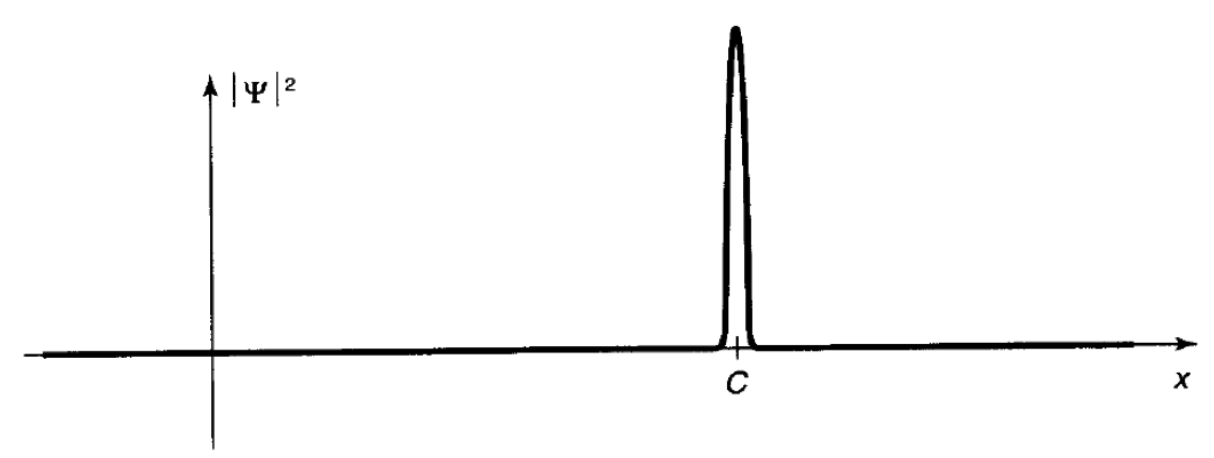
\includegraphics[width=0.5\linewidth]{sections/fig/WavefunctionCollapse.png}
			\caption{波函数坍缩示意图} 
			\label{fig.WavefunctionCollapse}
		\end{figure}
	\section{概率}
		已知j的概率分布,定义j的函数的平均值
		\begin{equation}
		\langle f(j)\rangle=\sum_{0}^{\infty} f(j) P(j)
		\end{equation}
		给出方差的定义和重要的一个定理
		%方差equ
			\begin{equation}
			\sigma^{2} \equiv\left\langle(\Delta j)^{2}\right\rangle
			\end{equation}
			\begin{equation}
			\begin{aligned}
			\sigma^{2} &=\left\langle(\Delta j)^{2}\right\rangle=\sum(\Delta j)^{2} P(j)=\sum(j-\langle j\rangle)^{2} P(j) \\
			&=\sum\left(j^{2}-2 j\langle j\rangle+\langle j\rangle^{2}\right) P(j) \\
			&=\sum j^{2} P(j)-2\langle j\rangle \sum j P(j)+\langle j\rangle^{2} \sum P(j) \\
			&=\left\langle j^{2}\right\rangle-2\langle j\rangle\langle j\rangle+\langle j\rangle^{2}=\left\langle j^{2}\right\rangle-\langle j\rangle^{2} .
			\end{aligned}
			\end{equation}
		上式取平方根,有$\sigma=\sqrt{\left\langle j^{2}\right\rangle-\langle j\rangle^{2}}$
	\section{归一化}
		波函数的统计诠释要求下式必须成立
		\begin{equation}
			\int_{-\infty}^{\infty}|\Psi(x, t)|^{2} d x=1
		\end{equation}
		薛定谔方程本身有着不同的特性,会自动保持波函数的归一化,下面给出证明:

		我们首先计算
		\begin{equation}
		\label{eq.1_1_0}
			\frac{d}{d t} \int_{-\infty}^{\infty}|\Psi(x, t)|^{2} d x=\int_{-\infty}^{\infty} \frac{\partial}{\partial t}|\Psi(x, t)|^{2} d x
		\end{equation}
		根据偏导数给出方程右边形式:
		\begin{equation}
		\label{eq.1_1_1}
			\frac{\partial}{\partial t}|\Psi|^{2}=\frac{\partial}{\partial t} \Psi^{*} \Psi=\Psi^{*} \frac{\partial \Psi}{\partial t}+\frac{\partial \Psi^{*}}{\partial t} \Psi
		\end{equation}
		将薛定谔方程写做
		\begin{equation}
			\frac{\partial \Psi}{\partial t}=\frac{i \hbar}{2 m} \frac{\partial^{2} \Psi}{\partial x^{2}}-\frac{i}{\hbar} V \Psi
		\end{equation}
		同时给出方程复共轭的形式
		\begin{equation}
			\frac{\partial \Psi^{*}}{\partial t}=-\frac{i \hbar}{2 m} \frac{\partial^{2} \Psi^{*}}{\partial x^{2}}+\frac{i}{\hbar} V \Psi^{*}
		\end{equation}
		代入式\ref{eq.1_1_1}可得
		\begin{equation}
		\label{eq.1_1_psi^2dt}
			\frac{\partial}{\partial t}|\Psi|^{2}=\frac{i \hbar}{2 m}\left(\Psi^{*} \frac{\partial^{2} \Psi}{\partial x^{2}}-\frac{\partial^{2} \Psi^{*}}{\partial x^{2}} \Psi\right)=\frac{\partial}{\partial x}\left[\frac{i \hbar}{2 m}\left(\Psi^{*} \frac{\partial \Psi}{\partial x}-\frac{\partial \Psi^{*}}{\partial x} \Psi\right)\right]
		\end{equation}
		则式\ref{eq.1_1_0}可直接写做
		\begin{equation}
			\frac{d}{d t} \int_{-\infty}^{\infty}|\Psi(x, t)|^{2} d x=\left.\frac{i \hbar}{2 m}\left(\Psi^{*} \frac{\partial \Psi}{\partial x}-\frac{\partial \Psi^{*}}{\partial x} \Psi\right)\right|_{-\infty} ^{\infty}
		\end{equation}
		即要求$x$趋于正负无限大的时候$\Psi (x,t)$必须趋于零————否则波函数式不可归一化的,所以得到
		\begin{equation}
			\frac{d}{d t} \int_{-\infty}^{\infty}|\Psi(x, t)|^{2} d x=0
		\end{equation}
	\section{动量}
		对于处于$\Psi$态的粒子(即处于“未观测态”的粒子),其x的期待值是
		\begin{equation}
		\label{eq.<x>}
		\langle x \rangle = \int_{-\infty}^{+\infty}x|\Psi (x,t)|^2 d x
		\end{equation}
		值得注意的是,这里不意味着对同一体系进行重复测量得到的平均值,而是对含有相同体系的一个系综中的不同体系的重复测量的平均值————如果对同一体系进行重复测量,第一次测量将导致分布的波函数坍缩。

		在函数随时间演化的过程中,我们更对$\langle x \rangle$发生的变化感兴趣,联立式\ref{eq.1_1_psi^2dt}和式\ref{eq.<x>},得到
		\begin{equation}
		\frac{d \langle x \rangle}{dt}=\int x \frac{\partial}{\partial t}|\Psi|^2 dx=\frac{i \hbar}{2m}\int x\frac{\partial}{\partial x}(\Psi^* \frac{\partial \Psi}{\partial x}-\frac{\partial \Psi^*}{\partial x}\Psi)dx
		\end{equation}
		利用分部积分公式得到\footnote{Unfinished}
		\begin{equation}
		\frac{d\langle x\rangle}{d t}=-\frac{i \hbar}{2 m} \int\left(\Psi^{*} \frac{\partial \Psi}{\partial x}-\frac{\partial \Psi^{*}}{\partial x} \Psi\right) d x
		\end{equation}
		对于上式,利用$\frac{\partial x}{\partial x}=1$,并丢掉了边界项,因为在无穷远处趋于零,再次分布积分得到
		\begin{equation}
		\langle v \rangle = \frac{d\langle x\rangle}{d t}=-\frac{i \hbar}{m} \int \Psi^{*} \frac{\partial \Psi}{\partial x} d x
		\end{equation}

		这里得到的是x期待值的“速度”。在量子力学中,本来就没有一个确切的速度定义————如果一个粒子没有一个确定的位置,就没有一个明确定义的速度,我们只能得到一个特定值的几率。

		在习惯中,我们使用动量表示:
		\begin{equation}
		\langle p \rangle = m \frac{d \langle x \rangle}{dt}=-i \hbar \int(\Psi^* \frac{\partial \Psi}{\partial x})dx
		\end{equation}
		我们把$\langle x \rangle$和$\langle p \rangle$的表示式写成更有启发意义的形式:
		\begin{equation}
		\begin{aligned}
		&\langle x\rangle=\int \Psi^{*}(x) \Psi d x \\
		&\langle p\rangle=\int \Psi^{*}\left(\frac{\hbar}{i} \frac{\partial}{\partial x}\right) \Psi d x
		\end{aligned}
		\end{equation}
		比较两个式子,我们可以发现计算任意量的期待值都可以将相应的算符放在$\Psi^*$和$\Psi$之间,然后求相应的积分,具体例子如下式\ref{eq.1_2_0}

		知道了位置和动量的量子力学表达,其他所有的经典力学量都可以表示为坐标和动量的函数。要计算这样的一个量的期待值,可以通过式
		\begin{equation}
		\label{eq.1_2_0}
		\langle Q(x, p)\rangle=\int \Psi^{*} Q\left(x, \frac{\hbar}{i} \frac{\partial}{\partial x}\right) \Psi d x
		\end{equation}

		请读者尝试求出动能的期待值\footnote{答案是
		\begin{equation}
		\langle T\rangle=-\frac{\hbar^{2}}{2 m} \int \Psi^{*} \frac{\partial^{2} \Psi}{\partial x^{2}} d x
		\end{equation}}

	\section{不确定原理}
		在直观感受上格里菲斯版的量子力学中给出的\textbf{绳的类比}相当的直观。\begin{figure}[H]
				\centering
				\subfigure[具有很好的波长定义,但是位置无法确定]{
				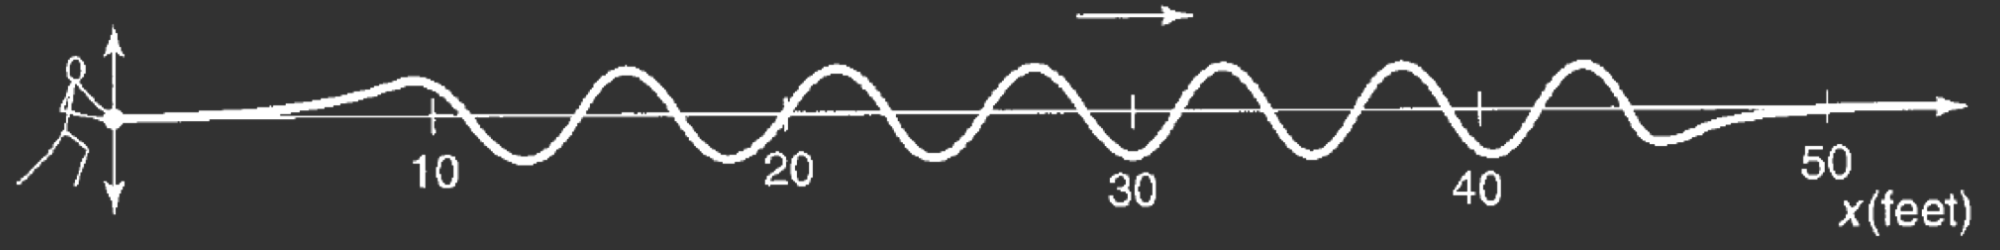
\includegraphics[width=0.7\linewidth]{sections/fig/UncertaintyI.png}
				}
				\quad
				\subfigure[具有很好的位置定义,但是波长无法定义]{
				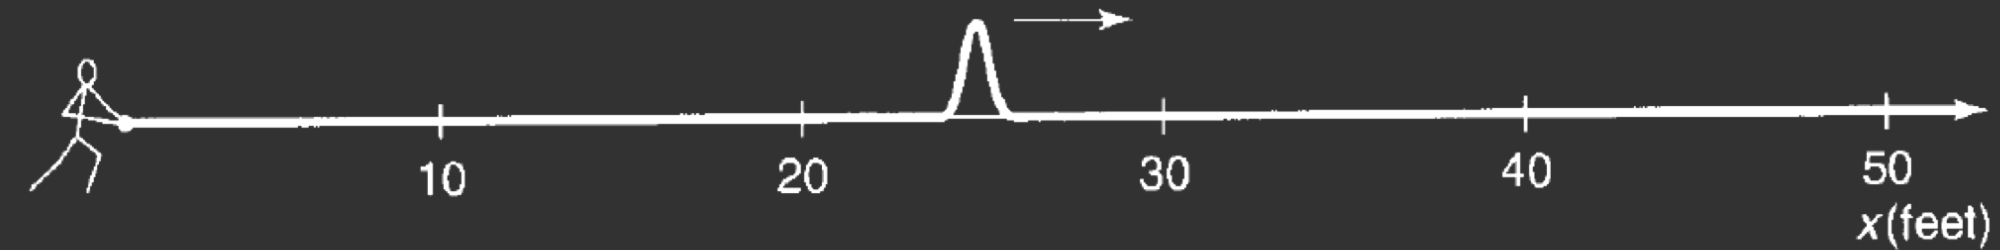
\includegraphics[width=0.7\linewidth]{sections/fig/UncertaintyII.png}
				}
				\caption{不确定性原理}
				\end{figure}

		粒子的动量同$\Psi$波长的联系由德布罗意公式给出。在这里我们不加证明的给出Heisenberg不确定原理,我们将在后面证明这个关系\footnote{Unfinished},在定量上有(其中中$\sigma_x$和$\sigma_p$分别是x和p的标准差)
			\begin{equation}
			\sigma_{x} \sigma_{p} \geq \frac{\hbar}{2}
			\end{equation}
	\chapter{定态薛定谔方程}
	\section{定态}
	对于薛定谔方程
	\begin{equation}
	i \hbar \frac{\partial \Psi}{\partial x}=-\frac{\hbar^{2}}{2 m} \frac{\partial^{2} \Psi}{\partial x^{2}}+V \Psi
	\end{equation}
	在学习阶段,我们研究的绝大部分情况下都会假设V是不含时间的。在这种情况下薛定谔方程可以通过分离变量法求解:我们寻找乘积形式的解
	\begin{equation}
	\Psi(x,t)=\psi(x) \varphi(t)
	\end{equation} 
	代入上式通过变形得到
	\begin{equation}
	i \hbar \psi(x) \varphi^{\prime}(t)= -\frac{\hbar^2}{2m}\psi^{\prime \prime}(x) \varphi(t)+V \psi(x)\varphi(t)
	\end{equation}
	将方程两边同时除以$\psi(x) \varphi(t)$,并将常数令为E,得到
	\begin{align}
	\label{eq.2_1_1}
	i \hbar \frac{\varphi^{\prime}(t)}{\varphi(t)}&=E \quad \Rightarrow \quad \frac{d \varphi(t)}{d t}=-\frac{i E}{\hbar} \varphi(t) \\
	\label{eq.2_1_2}
	-\frac{\hbar^{2}}{2 m} \frac{\psi^{\prime \prime}(x)}{\psi(x)}+V&=E \quad \Rightarrow \quad -\frac{\hbar^{2}}{2 m} \frac{d^{2} \psi}{d x^{2}}+V \psi=E \psi
	\end{align}
	其中式\ref{eq.2_1_1}能够解出得到
	\begin{equation}
	\varphi(t) = \exp(iEt/\hbar)
	\end{equation}
	第二式\ref{eq.2_1_2}即为\textbf{定态(time-independent)薛定谔方程},如果不指定V的话我们就无法进一步求它的解

	我们下面简述一下分离变量法在这里可行的原因
	\begin{enumerate}
	\item 虽然波函数本身和时间有关,但是计算几率密度的时候,时间因子相互抵消————在根据式\ref{eq.1_2_0}得到这时候任何一个期待值都是不含时的,我们可以直接用$\psi$来代替$\Psi$
		\begin{equation}
		|\Psi(x, t)|^{2}=\Psi^{*} \Psi=\psi^{*} e^{+i E t / \hbar} \psi e^{-i E t / \hbar}=|\psi(x)|^{2}
		\end{equation}
	\item 它们都是具有确定总能量的态,对于哈密顿量
		\begin{equation}
		H(x, p)=\frac{p^{2}}{2 m}+V(x)
		\end{equation}
	用动量的替换算符得到哈密顿量的替换算符
		\begin{equation}
		\hat{H}=-\frac{\hbar^{2}}{2 m} \frac{\partial^{2}}{\partial x^{2}}+V(x)
		\end{equation}
	这样定态薛定谔方程就可以直接写为
		\begin{equation}
		\hat{H} \psi=E \varphi
		\end{equation}
	
	\qquad 可以得到总能量的期望值便是E,这也是前面常数直接令为E的原因。我们验证这个结论,我们可以直接算出H的标准差
		\begin{equation}
		\sigma_{H}^{2}=\left\langle H^{2}\right\rangle-\langle H\rangle^{2}=E^{2}-E^{2}=0
		\end{equation}
	
	\qquad 这意味着每个样本有同样的值(分布没有弥散)————结论:分离变量解有这样一种性质, 总能量的每次测量结果是确定的值E
	\item 一般解是分离变量解的线性叠加,当然对于每个解都有相应的分量常数————\textbf{每个常数对应能量不同的波函数},一旦得到分离解就可以表示出一般解的形式
		\begin{equation}
		\Psi(x, t)=\sum_{n=1}^{\infty} c_{n} \psi_{n}(x) e^{-i E_{n} t / \hbar}
		\end{equation}
	\end{enumerate}

	下面简单总结一下,我们研究的一般问题是:\textbf{给定一个势V(x)和一个初始波函数$\Psi(x,0)$,要求出任何时刻的波函数。}我们一般会首先求出定态薛定谔方程,代入初始条件得到在$t=0$时解的线性组合
		\begin{equation}
		\Psi(x, 0)=\sum_{n=1}^{\infty} c_{n} \psi_{n}(x)
		\end{equation}
	通过上式找到合适的常数之后,加上含时项便得到
	\begin{equation}
	\label{eq.2_1_3}
	\boxed{\Psi(x, t)=\sum_{n=1}^{\infty} c_{n} \psi_{n}(x) e^{-i E_{n} t / \hbar}=\sum_{n=1}^{\infty} c_{n} \Psi_{n}(x, t)}
	\end{equation}
	需要强调的是,要区分开定态解和一般解,一般解中不同的定态有不同的能量,因为其时间因子不能相互抵消。
\section{一维无限深方势阱}
	如果粒子在势能分布满足
	\begin{equation}
	V(x)=\left\{\begin{array}{cl}
	0, & 0 \leq x \leq a \\
	\infty, & else \ x
	\end{array}\right.
	\end{equation}
	的区域运动,一个粒子在这样的势能中除了在两个端点外都是自由的,在端点处有无穷大的力限制它逃逸,称为一维无限深势阱。

	我们可以直观的得到,在势阱外找到粒子的几率是零。在势阱内$V(x)=0$,我们有定态薛定谔方程
	\begin{equation}
	\hat{H} \psi= -\frac{\hbar^2}{2m} \frac{\partial^2 \psi}{\partial x^2}= E \psi
	\end{equation}
	求解该ODE,得到通解
	\begin{align}
	\psi &= A \sin{\mu x}+B \cos{\mu x} \\
	\mu &= \sqrt{\frac{2mE}{\hbar^2}}
	\end{align}
	代入边界条件$\psi(0)=\psi(a)=0$,求解得到
	\begin{equation}
	\mu a = \pm n \pi \ , n \in \mathbb{N}^*
	\end{equation}

	考虑到关系$\sin(-x)=-\sin(x)$,上式可以将正负号合并为
	\begin{equation}
	\mu a = n \pi \ , n \in \mathbb{N}^*
	\end{equation}
	这个无限深势阱内的前三个定态
	\begin{figure}[H]
		\centering  % width栏调节相对行宽的大小
		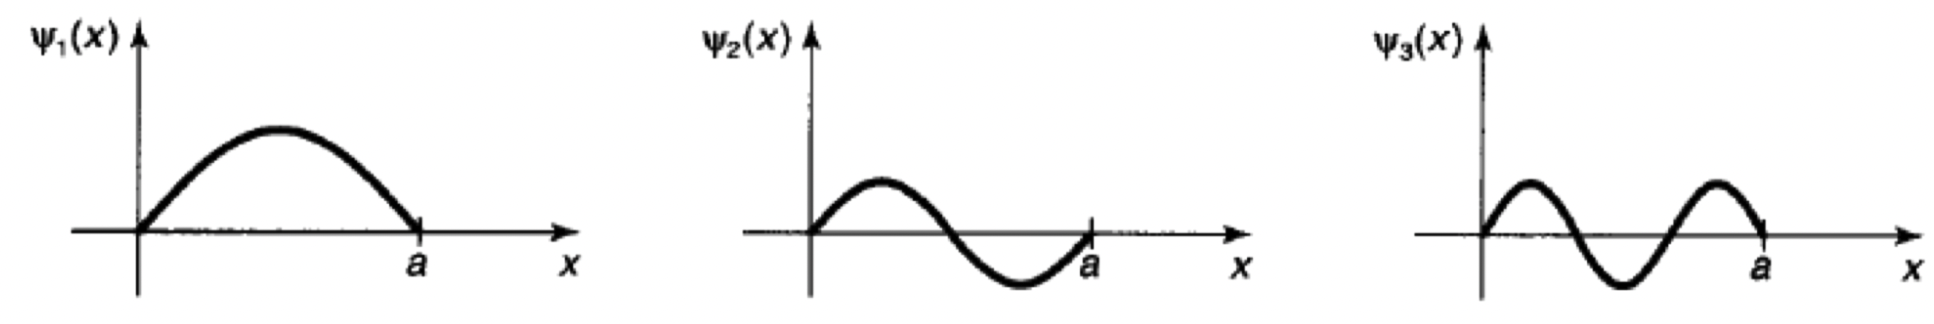
\includegraphics[width=0.7\linewidth]{sections/fig/1DInfiniteSquarePotential_1.png}
		\caption{无限深势阱内的前三个定态示意图} % 图片添加注释
		\label{fig.1DInfiniteSquarePotential_1}
	\end{figure}

	代入原式,得到能量之间的关系
	\begin{equation}
	\label{eq.2_2_1}
	\boxed{E= \frac{n^2 \pi^2 \hbar^2}{2m a^2} \ , n \in \mathbb{N}^*}
	\end{equation}

	上面的求解过程有一个有趣的现象,x轴两端的边界条件没有确定系数的值,反而确定了常数$\mu$可能的取值,从而得到了式\ref{eq.2_2_1}。这里能量的取值和经典情况有所不同,一个量子化的粒子在一维无限深势阱中的能量不能是任意的,它只是这些特殊的许可值,而这一结果(即能量量子化)也是定态薛定谔方程边界条件所要求的结果。

	为求出系数A,利用归一化条件
	\begin{equation}
	\int_{0}^{a}|A|^{2} \sin ^{2}(k x) d x=|A|^{2} \frac{a}{2}=1
	\end{equation}

	得到定态薛定谔方程在阱内的解是
	\begin{equation}
	\boxed{\psi_{n}(x)=\sqrt{\frac{2}{a}} \sin \left(\frac{n \pi}{a} x\right)}
	\end{equation}

	有前文所述,解定态薛定谔方程会得到一个无限的解集(前三个定态解画在了图\ref{fig.1DInfiniteSquarePotential_1}中,\textbf{我们总结一下这些解的性质}
	\begin{enumerate}
	\item 它们看起来像在一个长度为a的弦上的驻波;$\psi_1$具有最低的能量,称为基态;其它态的能量正比于$n^2$增加,称为激发态
	\item 它们相对于势阱的中心是奇偶交替的:$\psi_1$是偶函数,$\psi_2$是奇函数,$\psi_3$是偶函数,依次类推
	\item 随着能量的增加,态的节点(与x轴交点)数逐次增1;$\psi_1$没有(端点不计),$\psi_2$有一个,$\psi_3$有两个,依次类推
	\item 它们是相互正交的,即满足当$m \neq n$时
			\begin{equation}
			\int \psi_{\mathrm{m}}^{*}(\mathrm{x}) \psi_{\mathrm{n}}(\mathrm{x}) d x=0
			\end{equation}
		  证明在脚注中给出\footnote{证明如下\begin{equation*}
									\begin{aligned}
									\int \psi_{\mathrm{m}}{ }^{*} (x) \psi_{\mathrm{n}}(x) d x&=\frac{2}{a} \int_{0}^{a} \sin \left(\frac{m \pi}{a} x\right) \sin \left(\frac{\mathrm{n} \pi}{a} x\right) d x \\
									&=\frac{1}{a} \int_{0}^{a}\left[\cos \left(\frac{m-n}{a} \pi x\right)-\cos \left(\frac{m+n}{a} \pi x\right)\right] d x \\
									&=\left.\left\{\frac{1}{(m-n) \pi} \sin \left(\frac{m-n}{a} \pi x\right)-\frac{1}{(m+n) \pi} \sin \left(\frac{m+n}{a} \pi x\right)\right\}\right|_{0} ^{a} \\
									&=\frac{1}{\pi}\left\{\frac{\sin [(m-n) \pi]}{(m-n)}-\frac{\sin [(m-n) \pi]}{(m-n)}\right\}=0 .
									\end{aligned}
									\end{equation*}}

		   事实上,如果考虑$m=n$的情况,我们就可以把正交性和归一性写在一起
		   \begin{equation}
				\boxed{\int \psi_{m}{ }^{*}(x) \psi_{n}(x) d x=\delta_{m n}}
		   \end{equation}
	\item 它们是完备的。即任意一个函数f(x)都可以用它们的线性迭加来表示
			\begin{equation}
				f(x)=\sum_{n=1}^{\infty} c_{n} \psi_{n}(x)=\sqrt{\frac{2}{a}} \sum_{n=1}^{\infty} c_{n} \sin \left(\frac{n \pi}{a} x\right)
			\end{equation}
			不难看出,上式即为f(x)的傅立叶展开式,可以通过正交归一性求得任意式的系数
			\begin{equation}
				\boxed{c_{n}=\int \psi_{\mathrm{n}}^{*}(\mathrm{x}) f(x) d x}
			\end{equation}
	\end{enumerate}

	上述的性质不只在无限深势阱的情况下有效:只要势是对称的,第二个形式就成立;对于其他性质,对于任何势都是普适的,但是证明可能会比较繁琐,在此省略。

	我们的目的是求解无限深势阱的波函数的解,利用前文式\ref{eq.2_1_3},我们加上含时项,得到波函数的定态解为
	\begin{equation}
		\Psi_{n}(x, t)=\sqrt{\frac{2}{a}} \sin \left(\frac{\mathrm{n} \pi}{a} x\right) e^{-i\left(n^{2} \pi^{2} \hbar / 2 m a^{2}\right) t}
	\end{equation}
	含时薛定谔方程的一般解是定态解的迭加
	\begin{equation}
		\Psi(x, t)=\sum_{n=1}^{\infty} c_{n} \sqrt{\frac{2}{a}} \sin \left(\frac{n \pi}{a} x\right) e^{-i\left(n^{2} \pi^{2} \hbar / 2 m a^{2}\right) t}
	\end{equation}
	代入初始的波函数,我们可以通过调整$c_n$系数的值来满足任意初始波函数$\Psi(x,0)$————${\psi_n}$的完备性可以保证上述的成立,我们也同样可以利用正交归一性得到相应的待定系数
	\begin{equation}
		c_{n}=\sqrt{\frac{2}{a}} \int_{0}^{a} \sin \left(\frac{n \pi}{a} x\right) \Psi(x, 0) d x
	\end{equation}

	有了这个波函数,就可以用第一节所学的方法来计算任何一个我们有兴趣的力学量。这种步骤对任何势能函数都是一样的,所不同的仅是$\psi$ 的函数形式和所允许的能量值满足的方程。
\section{谐振子}
	经典谐振子的模型是一个质量为 m 物体挂在一个力常数为 k 的弹簧上。其运动由胡克(Hooke)定律决定(忽略摩擦力),它的解是
	\begin{align}
		x(t)&=A \sin (\omega t)+B \cos (\omega t) \\
		\omega &\equiv \frac{k}{m}
	\end{align}

	由于谐振子在偏离较多的位置胡克定律就是失效,我们一般在势能极小值做泰勒展开
	\begin{equation}
		V(x)=V\left(x_{0}\right)+V^{\prime}\left(x_{0}\right)\left(x-x_{0}\right)+\frac{1}{2} V^{\prime \prime}\left(x_{0}\right)\left(x-x_{0}\right)^{2}+\cdots
	\end{equation}
	并设置相应的势能零点\footnote{可参见理论力学中微振动一节},就可以得到形如下式
	\begin{equation}
		V(x) \cong \frac{1}{2} V^{\prime \prime}\left(x_{0}\right)\left(x-x_{0}\right)^{2}
	\end{equation}

	我们考虑量子力学问题————要求解势能为
	\begin{equation}
		V(x)=\frac{1}{2} \omega^{2} x^{2}
	\end{equation}
	时的定态薛定谔方程。我们已经知道,只需解定态薛定谔方程就足够了
	\begin{equation}
	\label{eq.2_3_1}
		-\frac{\hbar^{2}}{2 m} \frac{d^{2} \psi}{d x^{2}}+\frac{1}{2} m \omega^{2} x^{2}=E \psi
	\end{equation}

	对于这个问题有两种,第一种是幂级数法直接求解微分方程,第二种是巧妙的代数方法。在这里我们先使用代数方法求解

	\subsection{代数法}
		我们用更具有启发性的形式改写式\ref{eq.2_3_1}
		\begin{equation}
			\frac{1}{2 m}\left[\hat{p}^{2}+(m \omega x)^{2}\right] \psi=E \psi
		\end{equation}
		求解的基本思想是分解哈密顿算符
		\begin{equation}
			\hat{H}=\frac{1}{2 m}\left[\hat{p}^{2}+(m \omega x)^{2}\right]
		\end{equation}
		如果只是数字关系,可以直接进行分解
		\begin{equation}
			u^{2}+v^{2}=(i u+v)(-i u+v)
		\end{equation}

		但是对于算符的运算需要考虑不同的运算次序带来的影响(不同的顺序对算符运算有着影响),为找出衡量算符能否交换的一个量度,我们检验这样的一个量
		\begin{equation}
			a_{\pm} \equiv \frac{1}{\sqrt{2 \hbar m \omega}}(\mp i p+m \omega x)
		\end{equation}
		(前面的因子是为了使计算的结果更加的优美)

		我们给出两者的积$a_- a_+$
		\begin{equation}
		\label{eq.2_3_2}
			\begin{aligned}
			a_{-} a_{+} &=\frac{1}{2 \hbar m \omega}(i p+m \omega x)(-i p+m \omega x) \\
			&=\frac{1}{2 \hbar m \omega}\left[p^{2}+(m \omega x)^{2}-i m \omega(x p-p x)\right]
			\end{aligned}
		\end{equation}
		正如预期,有一个额外项,即涉及到$(xp-px)$————我们称为x与p的对易子,这便是衡量算符是否能够交换的量度。我们简记为,A和B的对易子
		\begin{equation}
		[A,B]=AB-BA
		\end{equation}
		现在将式\ref{eq.2_3_2}改写为,
		\begin{equation}
			a_{-} a_{+}=\frac{1}{2 \hbar m \omega}\left[p^{2}+(m \omega x)^{2}\right]-\frac{i}{2 \hbar}[x, p]
		\end{equation}
		接下来需要求出对易子$[x,p]$,注意:我们引入一个待定函数f(x)使这一抽象的运算变得更具像化,在计算的最后再撤去待定函数,对于当前的这一个例子吗,我们有
		\begin{equation}
			[x, p] f(x)=\left[x \frac{\hbar}{i} \frac{d}{d x}(f)-\frac{\hbar}{i} \frac{d}{d x}(x f)\right]=\frac{\hbar}{i}\left(x \frac{d f}{d x}-x \frac{d f}{d x}-f\right)=i \hbar f(x)
		\end{equation}
		得到
		\begin{equation}
		\boxed{[x, p]=i \hbar}
		\end{equation}
		这个可爱的结果就是\textbf{正则对易关系}\footnote{量子力学中很多神奇的结论都源于坐标和动量不对易这个事实上去。如果将该关系作为量子力学的公理,也可导出$\hat{p}=(\hbar/i)d/dx$}

		利用上面的关系,我们就可以把式\ref{eq.2_3_2}改写为
		\begin{align}
		a_{-} a_{+}&=\frac{1}{\hbar \omega} H+\frac{1}{2} \\
		\label{eq.2_3_3} H&=\hbar \omega\left(a_{-} a_{+}-\frac{1}{2}\right)
		\end{align}
		值得注意的是,式\ref{eq.2_3_3}的写法仍然欠缺一些一般性————对易项前的符号与$a_-$和$a_+$的顺序有关,更一般的,我们将谐振子的定态薛定谔方程记为
		\begin{equation}
			\hbar \omega\left(a_{\pm} a_{\mp} \pm \frac{1}{2}\right) \psi=E \psi
		\end{equation}

		接下来的步骤就是代数法求解的关键所在————通过阶梯算符生成新解,即通过升降能量的方式得到其他能量的解。我们首先给出关键性的一个断言,并随后给出证明:\textbf{断言如果$\Psi$能够满足能量为$E$的薛定谔方程,则$a_+ \psi$满足能量为($E+\hbar \omega$)的薛定谔方程;$a_- \psi$满足能量为($E-\hbar \omega$)的薛定谔方程。}即
		\begin{equation}
			\begin{aligned}
			H\left(a_{+} \psi\right)&=(E+\hbar \omega)\left(a_{+} \psi\right) \\
			H\left(a_{-} \psi\right)&=(E-\hbar \omega)\left(a_{-} \psi\right)
			\end{aligned}	
		\end{equation}
		
		下面我们给出证明,在过程中需要注意,算符对于常数来说没有次序的区别,可以直接使用交换律————即算符对任意常数都是对易的
		\begin{equation}
			\begin{aligned}
			H\left(a_{+} \psi\right) &=\hbar \omega\left(a_{+} a_{-}+\frac{1}{2}\right)\left(a_{+} \psi\right)=\hbar \omega\left(a_{+} a_{-} a_{+}+\frac{1}{2} a_{+}\right) \psi \\
			&=\hbar \omega a_{+}\left(a_{-} a_{+}+\frac{1}{2}\right) \psi=a_{+}\left[\hbar \omega\left(a_{+} a_{-}+1+\frac{1}{2}\right) \psi\right] \\
			&=a_{+}(H+\hbar \omega) \psi=a_{+}(E+\hbar \omega) \psi=(E+\hbar \omega)\left(a_{+} \psi\right) .
			\end{aligned}
		\end{equation}

		我们将$a_{\pm}$称为阶梯算符,可以通过一个解得到其他能态的解。但是根据这种说法,我们要考虑边界的问题,显然是不能一直使用降阶算符进行能态运算的————根据我们的常识,在基态的时候这一降阶的运算就会停止,导致这一结果的情况就是归一化条件的存在。它可能是零或者它的平方积分可能是无限大的,事实上它是前者,即基态的时候满足\footnote{Unfinished\_Why}
		\begin{equation}
			a_{-} \psi_{0}=0
		\end{equation}
		————这一情况决定了无法进一步使用降阶算符计算

		我们接下来代入$a_-$求解这一基态
		\begin{equation}
			\frac{1}{\sqrt{2 \hbar m \omega}}\left(\hbar \frac{d}{d x}+m \omega x\right) \psi_{0}=0
		\end{equation}
		改写为
		\begin{equation}
			\frac{d \psi_{0}}{d x}=-\frac{m \omega}{\hbar} x \psi_{0}
		\end{equation}
		很好求解该ODE
		\begin{equation}
			\int \frac{d \psi_{0}}{\psi}=-\frac{m \omega}{\hbar} \int x d x \Rightarrow \ln \psi_{0}=-\frac{m \omega}{2 \hbar} x^{2}+\text{常数}
		\end{equation}
		所以
		\begin{equation}
			\psi_{0}(x)=A e^{-\frac{m \omega}{2 \hbar} x^{2}}
		\end{equation}
		利用归一化求解系数A
		\begin{equation}
			1=|A|^{2} \int_{-\infty}^{\infty} e^{-m \omega x^{2} / \hbar} d x=|A|^{2} \sqrt{\frac{\pi \hbar}{m \omega}}
		\end{equation}
		得到$A^{2}=\sqrt{m \omega / \pi \hbar}$,因此
		\begin{equation}
			\boxed{\psi_{0}(x)=\left(\frac{m \omega}{\pi \hbar}\right)^{1 / 4} e^{-\frac{m \omega}{2 \hbar} x^{2}}}
		\end{equation}
		代入薛定谔方程就可以求解相应的能量

		然后我们就可以在基态的时候,通过反复使用升阶算符计算激发态,每一次增加能量为$\hbar \omega$
		\begin{equation}
			\boxed{\psi_{n}(x)=A_{n}\left(a_{+}\right)^{n} \psi_{0}(x), \quad E_{n}=\left(n+\frac{1}{2}\right) \hbar \omega}
		\end{equation}
	\subsection{解析法}
		我们重新考虑方程
			\begin{equation}
				-\frac{\hbar^{2}}{2 m} \frac{d^{2} \psi}{d x^{2}}+\frac{1}{2} m \omega^{2} x^{2} \psi=E \psi
			\end{equation}
		并尝试使用级数的方法去求解。

		为更直观的得到微分方程的解,我们尝试把方程化为
		\begin{equation}
			\frac{d^{2} \psi}{d \xi^{2}}=A \psi
		\end{equation}	
		的形式

		经过化简,我们得到
		\begin{equation}
			\frac{d^{2} \psi}{d \xi^{2}}=\left(\xi^{2}-K\right) \psi
		\end{equation}
		其中有
		\begin{equation}
			\xi \equiv \sqrt{\frac{m \omega}{\hbar}} x
		\end{equation}
		\begin{equation}
			K \equiv \frac{2 E}{\hbar \omega}
		\end{equation}
		其近似解为
		\begin{equation}
			\psi(\xi) \approx A e^{-\xi^{2} / 2}+B e^{+\xi^{2} / 2}
		\end{equation}


		我们的主要方向是求解上面的方程,并得到能量E可能的情况(即所有K可能的值),首先在$x \to \infty$时,$\xi \to \infty$,且$\psi \to 0$,所以相关的解可以化简为
		\begin{equation}
			\psi(\xi)=h(\xi) e^{-\xi^{2} / 2}
		\end{equation}

		代入定态薛定谔方程得到
		\begin{equation}
			\frac{d^{2} h}{d \xi^{2}}-2 \xi \frac{d h}{d \xi}+(K-1) h=0
		\end{equation}
		这是一个Legendre方程,按照数学物理方法中的结论,其中h的级数展开解有
		\begin{equation}
			h(\xi)=a_{0}+a_{1} \xi+a_{2} \xi^{2}+\cdots=\sum_{j=0}^{\infty} a_{j} \xi^{j}
		\end{equation}

		其截断时的特征值需要满足
		\begin{equation}
			K=2 n+1
		\end{equation}
		也即能量需要满足
		\begin{equation}
			E_{n}=\left(n+\frac{1}{2}\right) \hbar \omega, \quad n=0,1,2, \ldots \ldots
		\end{equation}

		这样写出归一化谐振子定态可以写为\footnote{其中还包含对归一化系数的小调整,具体可以参见教材}
		\begin{equation}
			\psi_{n}(x)=\left(\frac{m \omega}{\pi \hbar}\right)^{1 / 4} \frac{1}{\sqrt{2^{n} n !}} H_{n}(\xi) e^{-\xi^{2} / 2}
		\end{equation}
		H为Hermitian多项式。

		在这里补充一个结论,对于任何的谐振子定态有
\section{自由粒子}
	自由粒子(处处V(x)=0),在经典理论中意味着粒子做等速运动。我们沿用上一节谐振子的处理方式,将方程写作
	\begin{equation}
		\frac{d^{2} \psi}{d x^{2}}=-k^{2} \psi , 其中  k \equiv \frac{\sqrt{2 m E}}{\hbar}
	\end{equation}
	用指数形式表示其一般解等于
	\begin{equation}
		\psi(x)=A e^{i k x}+B e^{-i k x}
	\end{equation}
	现在对于无穷远处的情况没有办法限制:自由粒子可以具有任何正的能量值,我们加上标准的时间因子得到完整的波函数方程
	\begin{equation}
		\Psi(x, t)=A e^{i k\left(x-\frac{\hbar k}{2 m} t\right)}+B e^{-i k\left(x+\frac{\hbar k}{2 m} t\right)}
	\end{equation}

	我们可以看出上式的对称性——事实上,两个项分别代表向不同方向传播的波,因为其形式上只有符号的区别,我们可以将它们合并写成一项
	\begin{equation}
		\Psi_{k}(x, t)=A e^{i\left(k x-\frac{\hbar k^{2}}{2 m} t\right)}
	\end{equation}
	其中满足\footnote{这里需要说明的是,在该方程的解中,与经典粒子速度相匹配的是波包的群速度而非定态时的相速度}
	\begin{equation}
	k \equiv \pm \frac{\sqrt{2 m E}}{\hbar}, \quad\left\{\begin{array}{l}
	k>0 \Rightarrow \text { 向右传播 } \\
	k<0 \Rightarrow \text { 向左传播 }
	\end{array}\right.
	\end{equation}

	则自由粒子的“定态”是传播的波,其波长等于$\lambda=2 \pi /|k|$。

	我们发现自由粒子的波函数是不可归一化的
	\begin{equation}
		\int_{-\infty}^{\infty} \Psi_{k}^{*} \Psi_{k} d x=|A|^{2} \int_{-\infty}^{\infty} d x=|A|^{2}(\infty)
	\end{equation}

	该波函数用作线性叠加依然是有意义的,但是不可归一化说明自由粒子不能存在于一个定态——即没有一个确定的能量。在一般的波函数求解的问题中,会给定$t=0$时的初始状态,我们可以通过傅立叶逆变换得到
	\begin{equation}
		\phi(k)=\frac{1}{\sqrt{2 \pi}} \int_{-\infty}^{\infty} \Psi(x, 0) e^{-i k x} d x
	\end{equation}
\section{$\delta$函数势}
	\subsection{束缚态和散射态}
		薛定鄂方程的两类解恰好对应束缚态和散射态。这种区分在量子的范畴甚至更清晰, 因 为隧道效应(我们会马上讨论到)允许粒子 “渗透” 穿过任何有限的势垒, 所以最关键的是 无限远处的势:
		\begin{equation}
		\left\{\begin{array}{l}
		E<[V(-\infty) \text { 和 } V(\infty)] \Rightarrow \text { 束缚态, } \\
		E>[V(-\infty) \text { 或 } V(\infty)] \Rightarrow \text { 散射态. }
		\end{array}\right.
		\end{equation}
	\subsection{$\delta$函数势阱}
	\subsection{有限深方势阱}







	\chapter{形式理论}
	\section{Hilbert空间}
	在N维空间中,可以简单地用对应于N个正交归一基矢的分量,可以用行列矩阵来表示
	\begin{equation}
		|\alpha\rangle \rightarrow \mathbf{a}=\left(\begin{array}{l}
		a_{1} \\
		a_{2} \\
		\vdots \\
		a_{N}
		\end{array}\right)
	\end{equation}
	
	同样可以定义两个矢量的内积
	\begin{equation}
		\langle\alpha \mid \beta\rangle=a_{1}^{*} b_{1}+a_{2}^{*} b_{2}+\cdots a_{N}^{*} b_{N}
	\end{equation}

	矩阵变换可以写做
	\begin{equation}
		|\beta\rangle=T|\alpha\rangle \rightarrow \mathbf{b}=\mathbf{T a}=\left(\begin{array}{cccc}
		t_{11} & t_{12} & \cdots & t_{1 N} \\
		t_{21} & t_{22} & \cdots & t_{2 N} \\
		\vdots & \vdots & & \vdots \\
		t_{N 1} & t_{N 2} & \cdots & t_{N N}
		\end{array}\right)\left(\begin{array}{l}
		a_{1} \\
		a_{2} \\
		\vdots \\
		a_{N}
		\end{array}\right)
	\end{equation}

	将\textbf{所有在特定区域的平方可积函数的集合}
		\begin{equation}
			f(x) \quad \text { 满足 } \quad \int_{a}^{b}|f(x)|^{2} d x<\infty
		\end{equation}
	\textbf{构成的一个矢量空间,称为希尔伯特空间。}在量子力学中,波函数是处于希尔伯特空间中的。

	定义两个函数的内积
	\begin{equation}
		\langle f \mid g\rangle \equiv \int_{a}^{b} f(x)^{*} g(x) d x
	\end{equation}

	如果一个函数与自身的内积为 1 , 我们称之为归一化的; 如果两个函数的内积为 0 , 那 么这两个函数是正交的; 如果一组函数即是归一的也是相互正交的, 称之它们为正交归一的。
	\begin{equation}
		\left\langle f_{m} \mid f_{n}\right\rangle=\delta_{m v}
	\end{equation}
\section{可观测量}
	\subsection{Hermitian算符}
		对于一个可观测量,一次测量结果的期望值和多次测量的平均值应当相同
		\begin{equation}
			\langle\psi \mid \hat{Q} \psi\rangle=\langle\hat{Q} \psi \mid \psi\rangle
		\end{equation}
		我们称这样的算符为Hermitian算符,Hermitian算符的期望值是实数,可观测量由厄密算符表示。

		举个例子,我们可以证明动量算符是厄密算符\footnote{通常会采用到分部积分法}
		\begin{equation}
			\langle f \mid \hat{p} g\rangle=\int_{-\infty}^{\infty} f^{*} \frac{h}{i} \frac{d g}{d x} d x=\left.\frac{h}{i} f^{*} g\right|_{-\infty} ^{\infty}+\int_{-\infty}^{\infty}\left(\frac{h}{i} \frac{d f}{d x}\right)^{*} g d x=\langle\hat{p} f \mid g\rangle
		\end{equation}
	\subsection{定值态}
		通常的, 当你对全同体系组成的系综测量一个可观测量 $Q$, 每个体系都处于相同的状态 $\Psi$, 每 次测量并不能得到相同的结果——这就是量子力学中的不确定性问题: 是否能够制备一个态 使得每一次观测 $Q$ 都一定得到同样的值?如果你喜欢, 可以称这样的态为可观测量 $Q$ 的定值态。\footnote{实际上, 我们已经知道一个例子:哈密顿的定态是定值态:测量一个粒子处于定态 $\Psi_{n}$ 时的总能量, 必定得到相应的 “允许的” 能量 $E_{n}$}

		则对于
		\begin{equation}
			\hat{Q} \Psi=q \Psi
		\end{equation}
		称为算符$\hat{Q}$的本征值方程,q是对应的本征值。有时候两个(或者多个)线性独立的本征函数具有相同的本征值,这种情况称为谱的简并。

	\subsection{Hermitian算符的本征函数}
		对于厄密算符的本征函数(也即可观测的定值态)分成两类情况
			\begin{enumerate}
			\item 如果谱是连续的,那么本征函数是不可归一化的,并且不能代表可能的波函数 
			\item 如果谱是分立的,那么它们的本征值是实数且不同本征值的本征函数是正交的
			\end{enumerate}

		某些算符只有分立谱,某些算符只有连续谱,某些算符两者都具有。
			\subsubsection{分立谱}
				数学上厄密算符归一化的本征函数有两个性质,我们在前文也已经提到,这里在给出性质的同时给出证明
					\paragraph*{定理1:它们的本征值是实数\\}
						\par
						证明: 假设
						\begin{equation}
						\hat{Q} f=q f
						\end{equation}
						\begin{equation}
						\langle f \mid \hat{Q} f\rangle=\langle\hat{Q} f \mid f\rangle
						\end{equation}
						( $\hat{Q}$ 是厄密算符)。那么有
						\begin{equation}
						q\langle f \mid f\rangle=q^{*}\langle f \mid f\rangle
						\end{equation}
						( $q$ 是一个数, 所以它可以移出积分号外, 并且因为内积的左侧是右侧函 数的复共轭 (等式 3.6) 所以在右边 $q$ 也同样移出)但是 $\langle f \mid f\rangle$ 不能是 0 ( $f(x)=0$ 不是正当的本征函数), 所以 $q=q^{*}$, 因此 $q$ 是实数。证毕。
					\paragraph*{定理2:属于不同本征值的本征函数是正交的\\}
						\par
						证明:假设
						\begin{equation}
						\hat{Q} f=q f, \quad \hat{Q} g=q^{\prime} g
						\end{equation}
						$\hat{Q}$ 是厄密算符。则有 $\langle f \mid \hat{Q} g\rangle=\langle\hat{Q} f \mid g\rangle$, 所以
						\begin{equation}
						q^{\prime}\langle f \mid g\rangle=q^{*}\langle f \mid g\rangle
						\end{equation}
						(再次, 内积是存在的因为假定本征函数是位于希耳伯特空间内)。但是 $q$ 是 实数 (由定理 1), 所以如果 $q^{\prime} \neq q$ 那么必然有 $\langle f \mid g\rangle=0$.

				补充一个公理:\textbf{可观测量算符的本征函数是完备的,(在希尔伯特空间中)任何函数都可以用它们的线性迭加来表达)}
			\subsubsection{连续谱}
		\subsection{广义统计诠释}	
			

















	\chapter{三维空间中的量子力学}
	\chapter{全同粒子}
	\chapter{不含时微扰理论}
		\section{非简并微扰理论}
    \subsection{微扰的概念和一般表达形式}
        对于之前一些简单的势场(如一维无限深势阱),我们已经可以求出精确解,并且得到相应的能量本征值。记作
            \begin{equation}
                H^0 \psi_n^0 =E_n^0 \psi_n^0
            \end{equation}

        现在如果我们对这个势进行微小扰动(比如在势阱底部加入一个小的突起),我们期望可以找到一个新的本征函数和本征值:
            \begin{equation}
                \label{eq.6_1_2}
                H^0 \psi_n =E_n \psi_n^0
            \end{equation}

        微扰理论即是这样一套理论:它可以利用无微扰是的精确解去求出有微扰时候的近似解。

        我们可以将加入微扰项之后的哈密顿量表示为
            \begin{equation}
                \label{eq.6_1_3}
                H = H^0 + \lambda H'
            \end{equation}

        相应的,我们可以将能量和波函数也相应的展开\footnote{你可能对于这里$\lambda$的引入抱有疑问,事实上它也完全不是必须要引入的——它只是作为一个标定来提示我们各物理量的展开分别对应在多少幂次,具体例子可以参见https://www.zhihu.com/question/480216895/answer/2066207326,我们将会在后文给出不引入$\lambda$的推导方案}
        \begin{equation}
            \label{eq.6_1_4}
            \begin{aligned}
            \psi_{n} &=\psi_{n}^{0}+\lambda \psi_{n}^{1}+\lambda^{2} \psi_{n}^{2}+\cdots \\
            E_{n} &=E_{n}^{0}+\lambda E_{n}^{1}+\lambda^{2} \dot{E}_{n}^{2}+\cdots
            \end{aligned}
        \end{equation}
        
        将式\ref{eq.6_1_4}和\ref{eq.6_1_3}代入式\ref{eq.6_1_2}并合并同类项能够得到
        \begin{equation}    
            \label{eq.6_1_5}
            \begin{gathered}
            H^{0} \psi_{n}^{0}+\lambda\left(H^{0} \psi_{n}^{1}+H^{\prime} \psi_{n}^{0}\right)+\lambda^{2}\left(H^{0} \psi_{n}^{2}+H^{\prime} \psi_{n}^{1}\right)+\cdots \\
            =E_{n}^{0} \psi_{n}^{0}+\lambda\left(E_{n}^{0} \psi_{n}^{1}+E_{n}^{1} \psi_{n}^{0}\right)+\lambda^{2}\left(E_{n}^{0} \psi_{n}^{2}+E_{n}^{1} \psi_{n}^{1}+E_{n}^{2} \psi_{n}^{0}\right)+\cdots
            \end{gathered}
        \end{equation}

        由此可以推导出直到n次幂满足的等式关系
    \subsection{一级近似理论}
        由上节的式\ref{eq.6_1_5}可以得到
        \begin{equation}
            \label{eq.6_1_6}
            H^{0} \psi_{n}^{1}+H^{\prime} \psi_{n}^{0}=E_{n}^{0} \psi_{n}^{1}+E_{n}^{1} \psi_{n}^{0}
        \end{equation}

        将等式两端同时对$\psi_n^0$做内积运算,可以得到\footnote{虽然我们没有对算符H做出特殊的标注,但是请时刻记住算符的各项性质,在这里由于E是常数,所以它可以直接提出barket外面}
        \begin{equation}
            \left\langle\psi_{n}^{0} \mid H^{0} \psi_{n}^{1}\right\rangle+\left\langle\psi_{n}^{0} \mid H^{\prime} \psi_{n}^{0}\right\rangle=E_{n}^{0}\left\langle\psi_{n}^{0} \mid \psi_{n}^{1}\right\rangle+E_{n}^{1}\left\langle\psi_{n}^{0} \mid \psi_{n}^{0}\right\rangle
        \end{equation}
        注意其中的$H^0$和$E^0_n$项,经过简单的变换它们可以抵消掉,又根据$\left\langle\psi_{n}^{0} \mid \psi_{n}^{0}\right\rangle=1$可以得到
        \begin{equation}
            \label{eq.6_1_8}
            \boxed{E_{n}^{1}=\left\langle\psi_{n}^{0}\left|H^{\prime}\right| \psi_{n}^{0}\right\rangle}
        \end{equation}
        这是一级近似理论中的一个基本结果:在实际中也是量子力学最重要的方程。\textbf{它说明能量的一级修正就是微扰在非微扰态中的期待值}

        为更加直观的理解这个结论,我们以无微扰的无限深势阱波函数作为例子应用这个结论\footnote{Unfinished}

        下面我们着手解决波函数的一级修正,将式\ref{eq.6_1_6}重写
        \begin{equation}
            \label{eq.6_1_9}
            \left(H^{0}-E_{n}^{0}\right) \psi_{n}^{1}=-\left(H^{\prime}-E_{n}^{1}\right) \psi_{n}^{0}
        \end{equation}
        方程右边已经是已知函数,整个方程是关于$\psi^1_n$的非齐次微分方程。由于无微扰的波函数式完备的,可以表示出同一矢量空间内的任一波函数,我们就将$\psi^1_n$写为$\psi^0_n$的线性组合
        \begin{equation}
            \label{eq.6_1_10}
            \psi_{n}^{1}=\sum_{m \neq n} c_{m}^{(n)} \psi_{m}^{0}
        \end{equation}
        在求和时没有包含$m=n$项,因为当$\psi^1_n$满足式\ref{eq.6_1_9}时,由于$\psi^1_n$已经由$\psi^0_n$线性表出,则$\psi^0_n$显然成立,这样可以让我们简化$\psi^0_n$项。这样一来,只要我们求解出系数$c_m^n$,我们就可以得到波函数的一级近似值。

        将式\ref{eq.6_1_10}代入式\ref{eq.6_1_9}可以得到
        \begin{equation}
            \sum_{m \neq n}\left(E_{m}^{0}-E_{n}^{0}\right) c_{m}^{(n)} \psi_{m}^{0}=-\left(H^{\prime}-E_{n}^{1}\right) \psi_{n}^{0}
        \end{equation}
        同对能量的处理方式一样,我们将上式两边同时取$\psi_l^0$的内积,可以得到
        \begin{equation}
            \sum_{m \neq n}\left(E_{m}^{0}-E_{n}^{0}\right) c_{m}^{(n)}\left\langle\psi_{l}^{0} \mid \psi_{m}^{0}\right\rangle=-\left\langle\psi_{l}^{0}\left|H^{\prime}\right| \psi_{n}^{0}\right\rangle+E_{n}^{1}\left\langle\psi_{l}^{0} \mid \psi_{n}^{0}\right\rangle
        \end{equation}
        取$l=n$的时候上式左边等于零,会退化到式\ref{eq.6_1_8},当我们取$l\neq n$时,可以得到
        \begin{equation}
            \left(E_{l}^{0}-E_{n}^{0}\right) c_{l}^{(n)}=-\left\langle\psi_{l}^{0}\left|H^{\prime}\right| \psi_{n}^{0}\right\rangle
        \end{equation}
        可以表示出系数
        \begin{equation}
            c_{m}^{(n)}=\frac{\left\langle\psi_{m}^{0}\left|H^{\prime}\right| \psi_{n}^{0}\right\rangle}{E_{n}^{0}-E_{m}^{0}}
        \end{equation}
        所以,
        \begin{equation}
        \label{eq.6_1_15}
            \boxed{\psi_{n}^{1}=\sum_{m \neq n} \frac{\left\langle\psi_{m}^{0}\left|H^{\prime}\right| \psi_{n}^{0}\right\rangle}{\left(E_{n}^{0}-E_{m}^{0}\right)} \psi_{m}^{0}}
        \end{equation}



	\chapter{含时微扰理论}
		


	\chapter{习题}
	%练习题文档%
\section{波函数习题}
	\paragraph*{\quad 假设从高度为h的悬崖上释放一块石头。当石头下落时,以随机的间隔,我摄取了一百万张照片。在每一张照片上我测量石头已经落下的距离。问:所有这些距离的平均值是多少?也就是说,下降距离的时间平均是多少?}
\end{document}